\documentclass[aps,pre,reprint,twocolumn,nofootinbib,superscriptaddress]{revtex4-2}

\usepackage{amsmath,amssymb,amsthm}
\usepackage{graphicx}
\usepackage{bm}
\usepackage{xurl}
\usepackage{xcolor}
\usepackage{hyperref}

\hypersetup{
    pdfauthor={Taishi Namba},
    pdftitle={The resolution gap in many degrees of freedom},
    pdfkeywords={coarse-graining, arrow of time, Fisher information, Gaussian states, coupled oscillators, matrix inequalities},
    hidelinks
}

\newtheorem{theorem}{Theorem}
\newtheorem{proposition}[theorem]{Proposition}
\newtheorem{lemma}[theorem]{Lemma}
\newtheorem{corollary}[theorem]{Corollary}
\newtheorem{conjecture}{Conjecture}
\newtheorem{observation}{Numerical result}
\theoremstyle{remark}
\newtheorem*{remark}{Remark}

\newcommand{\Sym}{\operatorname{Sym}}
\newcommand{\tr}{\operatorname{tr}}
\newcommand{\E}{\mathbb{E}}
% Draft marker for results that wait for stage M of the numerical study. Remove before release.
\newcommand{\pending}[1]{{\color{red}\textbf{[#1]}}}

\begin{document}

\title{The resolution gap in many degrees of freedom}

\author{Taishi Namba}
\email{neginyan@gmail.com}
\affiliation{Independent Researcher, Atsugi, Kanagawa, Japan}

\date{\today}

\begin{abstract}
Gaussian coarse-graining at resolution $\sigma$ turns the conserved Gibbs entropy of a Hamiltonian ensemble into a coarse-grained entropy that grows if and only if the resolution coarsens faster than a critical rate $R$. The largest symmetric strain rate $\kappa$ of the flow bounds $R$ for all Gaussian states, in any dimension, and for one degree of freedom the best Gaussian state stays below $\kappa$ by a resolution gap $2\sqrt{2\beta\kappa}\,\sigma$, where $\beta$ measures how fast the strain decreases away from its maximum. Here we ask how this gap depends on the number of degrees of freedom, for mechanical systems $H = |p|^2/2 + V(q)$. We prove that the averaged strain felt by a Gaussian state depends only on its spread in configuration space, so that spreading along momentum directions is free. We prove that the best Gaussian state has a gap of at most $\Gamma\sigma + O(\sigma^2)$ with $\Gamma = 2\tr[(B^{1/2}CB^{1/2})^{1/2}]$. Here $B$, minus one half of the Hessian in configuration space of the strain along the most stretching direction, says how fast that strain falls when the state spreads, and $C = \mathrm{diag}(2\kappa,\kappa,\dots,\kappa)$ prices the directions over which the observer must spread its focus. The coefficient does not grow with the number of degrees of freedom as such: uncoupled degrees of freedom cost nothing, and a coupled one costs in proportion to how strongly the maximal strain depends on it. For two pendulums with coupling $\varepsilon$ we obtain $\Gamma$ in closed form, with $\Gamma = 1 + \sqrt\varepsilon + \tfrac34\varepsilon + \tfrac18\varepsilon^{3/2} + O(\varepsilon^2)$. Numerically, the formula is the optimum over all Gaussian states: searches that assume no shape find the optimal state on their own and never go below it, and in thirteen systems the optimum agrees with $\Gamma$ to a relative $4\times10^{-8}$. Six of these systems, chains of three and four pendulums and pendulums with a product coupling, were predicted before they were optimized, with the predictions recorded and hashed in advance. Mixtures of Gaussians, which beat the best Gaussian state by several per cent in one degree of freedom, gain only $40$--$55\%$ as much in two at the same search effort, almost entirely by mixing in the plane of the most stretching mode. All statements and numbers are reproduced by openly available code.
\end{abstract}


\maketitle

\section{Introduction}
\label{sec:intro}

A Hamiltonian flow preserves the Gibbs entropy of every ensemble. An observer who sees the phase space only through a Gaussian window of width $\sigma$ sees instead the coarse-grained density $\rho_C = \rho * \mathcal N(0,\sigma^2 I)$, and its entropy $S_C$ can grow. In Ref.~\cite{namba2026arrow} the window was allowed to coarsen at a rate $r = \dot\sigma/\sigma$, and it was shown that
\begin{equation}
\frac{dS_C}{dt} = \sigma^2\,\tr F\,(r - R),
\label{eq:SC}
\end{equation}
with $F$ the Fisher matrix of $\rho_C$ and a critical rate $R$ that depends on the state. For linear flows the supremum of $R$ over all states is the largest symmetric strain rate $\kappa$ of the flow, and it was conjectured that $R \leq \kappa$ also for nonlinear flows.

In Ref.~\cite{namba2026gap} the conjecture was proved for all Gaussian states, in any dimension, through the identity
\begin{equation}
R = \frac{\tr(F\,\Sym\bar J)}{\tr F}, \qquad F = (S + \sigma^2 I)^{-1}, \qquad \bar J = \E[Df],
\label{eq:law}
\end{equation}
for a Gaussian state $\mathcal N(m,S)$ of a flow $f$. For one degree of freedom the best Gaussian state was found: a thin segment through the point of maximal strain, whose gap is
\begin{equation}
\kappa - R^* = 2\sqrt{2\beta\kappa}\,\sigma + O(\sigma^2),
\label{eq:gap1}
\end{equation}
where $\beta$ measures how fast the strain decreases away from its maximum. The gap is linear in $\sigma$: a finite resolution keeps a margin in the arrow of time. Mixtures of Gaussians reduce the gap by up to about $8\%$ but keep it proportional to $\sigma$~\cite{namba2026gap}.

The picture behind Eq.~\eqref{eq:gap1} is a compromise of the observer's focus. To feel the maximal strain, the observer must spend its Fisher information on the most stretching direction, which requires the state to be sharp across that direction and long along the others. A long state cannot stay at the point of maximal strain, so it feels less strain. With more degrees of freedom there are more directions along which the state must be long, and one might expect the gap to grow with their number.

This article shows that it does not, and identifies what the gap depends on instead. We restrict to mechanical systems $H = |p|^2/2 + V(q)$, the class that contains coupled oscillators and pendulums. Our results are the following.
\begin{enumerate}
\item The averaged strain felt by a Gaussian state depends only on the state's spread in configuration space (Proposition~\ref{prop:momentum}). Spreading along momentum directions is free.
\item The best Gaussian state has a gap of at most $\Gamma\sigma + O(\sigma^2)$, with the matrix formula $\Gamma = 2\tr[(B^{1/2}CB^{1/2})^{1/2}]$ (Theorem~\ref{thm:upper}). The strain-decay matrix $B$ is computed from the potential at the point of maximal strain; the cost matrix $C$ is universal. Degrees of freedom that do not affect the maximal strain do not enter.
\item For two coupled pendulums $\Gamma$ is explicit, and full optimizations over Gaussian states without any assumed shape find the state that the formula predicts, with the same gap to a relative $10^{-8}$ (Sec.~\ref{sec:coupled}). We therefore conjecture that $\Gamma$ is exact (Conjecture~\ref{conj:optimal}).
\item The formula predicts the gap of systems that played no part in its derivation. Predictions for chains of three and four pendulums and for a product coupling were recorded, with time and hash, before the optimization, and all six were confirmed (Sec.~\ref{sec:prediction}).
\item Mixtures, which beat Gaussian states in one degree of freedom, gain $40$--$55\%$ as much in two at equal search effort, almost entirely inside the plane of the most stretching mode; an empirical law for the reduction predicted two further couplings to within $6\%$ (Sec.~\ref{sec:mixtures}).
\end{enumerate}
Throughout, we separate what is proved from what is observed numerically.

\section{Setting}
\label{sec:setting}

We consider $H(q,p) = \tfrac12|p|^2 + V(q)$ on $\mathbb R^{2n}$ (or with $q$ on a torus), with $V$ six times continuously differentiable and its derivatives up to sixth order bounded. All examples in this article are trigonometric and satisfy this. The sixth order is needed only for the $O(\sigma^2)$ remainder in Theorem~\ref{thm:upper}, because the strain contains $V''$; with four continuous bounded derivatives the leading-order statements still hold, with $o(\sigma)$ in place of $O(\sigma^2)$ (Appendix~\ref{app:proofs}). The flow is $f = (p, -\nabla V)$ and
\begin{equation}
Df = \begin{pmatrix} 0 & I \\ -V'' & 0 \end{pmatrix}, \qquad
\Sym Df = \begin{pmatrix} 0 & M \\ M & 0 \end{pmatrix}, \qquad M(q) = \frac{I - V''(q)}{2}.
\label{eq:strain}
\end{equation}
The eigenvalues of $\Sym Df$ at $(q,p)$ are $\pm\mu_j(q)$, where $\mu_j(q)$ are the eigenvalues of $M(q)$, so the largest symmetric strain rate is $\sup_q \max_j|\mu_j(q)|$. We assume that it is attained on the positive side,
\begin{equation}
\kappa = \sup_q \lambda_{\max}(M(q)) \;\geq\; \sup_q\big(-\lambda_{\min}(M(q))\big),
\label{eq:kappa}
\end{equation}
so that $\kappa$ is the largest symmetric strain rate. This is no loss of generality. The reflection $O = \mathrm{diag}(I,-I)$, $p \mapsto -p$, maps Gaussian states to Gaussian states, with $F \mapsto OFO$, and $O\,\Sym\bar J\,O$ has $-\bar M$ in place of $\bar M$; since $R = \tr(F\Sym\bar J)/\tr F$ is invariant under this conjugation and depends on the flow only through $\bar M$, the problem with the maximum on the negative side is the problem with $M$ replaced by $-M$, that is, $V''$ replaced by $2I - V''$. The definitions and proofs below use $V$ only through $M$, so they apply with $e_+$ the eigenvector of $\lambda_{\min}$ and $g = -e_+^{\mathsf T}Me_+$. All examples in this article satisfy Eq.~\eqref{eq:kappa}; we checked this on grids over the torus.

\emph{Gaussian states.} A Gaussian state $\mathcal N(m,S)$ has $S \succeq 0$; we allow singular $S$, as in Ref.~\cite{namba2026gap}. Equation~\eqref{eq:law} remains valid for them: the coarse-grained density $\mathcal N(m, S + \sigma^2 I)$ is smooth for every $S \succeq 0$, and $\bar J = \E[Df]$ is an average over the state, which exists because $V''$ is bounded. Moreover $R$ is a continuous function of $S \succeq 0$: $F = (S+\sigma^2I)^{-1}$ is continuous, and so is $\bar J = \E[Df(m + S^{1/2}z)]$, $z \sim \mathcal N(0,I)$, by dominated convergence, since $S \mapsto S^{1/2}$ is continuous on $S \succeq 0$ and $Df$ is bounded and continuous. Hence, at every fixed $\sigma$, a singular state is the limit of non-degenerate states $S + \eta I$, $\eta \to 0$, with the same limit of $R$, and the supremum $R^*$ is the same whether or not singular states are admitted. A singular state can thus be read as a shorthand for a non-degenerate one of arbitrarily small extra width.

\emph{Assumption.} The supremum is attained at a point $q_0$, and $\lambda_{\max}(M(q_0)) = \kappa$ is a simple eigenvalue. We write $e_1 = e_+$ for its unit eigenvector and $e_2,\dots,e_n$ for the other eigenvectors of $M(q_0)$, with eigenvalues $\mu_j < \kappa$.

\emph{Frame.} At $q_0$ we use the orthonormal basis of phase space
\begin{equation}
v = \tfrac{1}{\sqrt2}(e_+, e_+),\quad w = \tfrac{1}{\sqrt2}(e_+, -e_+),\quad a_j = (e_j, 0),\quad b_j = (0, e_j),
\label{eq:frame}
\end{equation}
$j = 2,\dots,n$. The vector $v$ is the most stretching direction of $\Sym Df$ (eigenvalue $\kappa$) and $w$ its contracting partner (eigenvalue $-\kappa$); $a_j$ and $b_j$ are the configuration and momentum directions of the other modes.

\emph{Strain-decay matrix.} Let $g(q) = e_+^{\mathsf T} M(q)\, e_+$, the strain along the fixed direction $e_+$. Since $g(q) \leq \lambda_{\max}(M(q)) \leq \kappa = g(q_0)$, the function $g$ has a maximum at $q_0$, so
\begin{equation}
B_q = -\tfrac12\nabla^2 g(q_0) = \tfrac14\nabla^2_q\big[e_+^{\mathsf T}V''(q)\,e_+\big]_{q_0} \succeq 0 .
\label{eq:Bq}
\end{equation}
The configuration-space parts of $w$ and $a_j$ are $e_+/\sqrt2$ and $e_j$. Collecting them in $P = (e_+/\sqrt2, e_2, \dots, e_n)$, we define the $n\times n$ matrices
\begin{equation}
B = P^{\mathsf T} B_q P, \qquad C = \mathrm{diag}(2\kappa, \kappa, \dots, \kappa),
\label{eq:BC}
\end{equation}
in the basis $(w, a_2, \dots, a_n)$, and the coefficient
\begin{equation}
\Gamma = 2\tr\big[(B^{1/2} C B^{1/2})^{1/2}\big] = 2\tr\big[(C^{1/2} B C^{1/2})^{1/2}\big].
\label{eq:Gamma}
\end{equation}
In words: $B$ says how fast the strain felt along $e_+$ falls when the state spreads in configuration space, and $C$ says how much Fisher information is wasted in each direction, measured against $\kappa$. Along $w$ the strain is $-\kappa$, a loss of $2\kappa$; along $a_j$ it is $0$, a loss of $\kappa$.

For one degree of freedom $P = 1/\sqrt2$, $B = \tfrac12 B_q$ and $C = 2\kappa$. With $\lambda(q) = \kappa - b(q-q_0)^2 + \dots$ near the maximum, $B_q = b$, and Eq.~\eqref{eq:Gamma} gives $\Gamma = 2\sqrt{2\kappa b/2} = 2\sqrt{2\beta\kappa}$ with $\beta = b/2$, the coefficient of Eq.~\eqref{eq:gap1}. For the pendulum $V = -\cos q$, $q_0 = \pi$, $\kappa = 1$, $b = 1/4$ and $\Gamma = 1$.

\section{Momentum directions are free, and an upper bound on the gap}
\label{sec:upper}

For a Gaussian state $\mathcal N(m,S)$ write $S_{qq}$ for its covariance in configuration space and $\bar M = \E[M(q)]$, $q \sim \mathcal N(m_q, S_{qq})$. Then $\bar J = \E[Df]$ has $\Sym\bar J = \begin{pmatrix} 0 & \bar M \\ \bar M & 0\end{pmatrix}$, and Eq.~\eqref{eq:law} reads
\begin{equation}
\kappa - R = \frac{\tr\big(F\,(\kappa I - K)\big)}{\tr F}, \qquad K = \Sym\bar J, \quad F = (S+\sigma^2I)^{-1}.
\label{eq:gaplaw}
\end{equation}

\begin{proposition}[Momentum directions are free]
\label{prop:momentum}
For $H = |p|^2/2 + V(q)$, the averaged strain $K$ of a Gaussian state depends on its covariance $S$ only through $S_{qq}$. Spreading the state along a pure momentum direction changes $F$ but not $K$.
\end{proposition}

\begin{proof}
$Df$ depends on $(q,p)$ only through $V''(q)$, so its average over $\mathcal N(m,S)$ is an average over the marginal law of $q$, which is $\mathcal N(m_q, S_{qq})$.
\end{proof}

In the picture of the observer's focus: the strain is felt in configuration space, while the focus is spent in phase space. A state that is long in momentum is not penalized by the strain, and the Fisher information it loses along that direction is small because the direction is long. This is why the $b_j$ do not appear in Eq.~\eqref{eq:BC}.

\begin{lemma}[Matrix identity]
\label{lem:matrix}
For $B \succeq 0$ and $C \succ 0$,
\begin{equation}
\inf_{T \succ 0}\;\big[\tr(BT) + \tr(CT^{-1})\big] = 2\tr\big[(C^{1/2}BC^{1/2})^{1/2}\big].
\label{eq:matrix}
\end{equation}
If $B \succ 0$ the infimum is attained at $T_* = C^{1/2}(C^{1/2}BC^{1/2})^{-1/2}C^{1/2}$.
\end{lemma}

The proof is in Appendix~\ref{app:proofs}. For $1\times1$ matrices it is $bt + c/t \geq 2\sqrt{bc}$, the balance that produced Eq.~\eqref{eq:gap1}.

\begin{theorem}[Upper bound on the gap of the best Gaussian state]
\label{thm:upper}
Under the assumption of Sec.~\ref{sec:setting}, for every $T \succ 0$ in the basis $(w, a_2,\dots,a_n)$ consider the Gaussian state with mean $(q_0, 0)$ and covariance
\begin{equation}
S = \sigma \sum_{i,j} T_{ij}\, u_i u_j^{\mathsf T} + \sum_{j=2}^n b_j b_j^{\mathsf T}, \qquad (u_1,\dots,u_n) = (w, a_2, \dots, a_n).
\label{eq:family}
\end{equation}
It has zero width along $v$, width of order $\sqrt\sigma$ along $w$ and the $a_j$, and width $1$ along the $b_j$. Its critical rate satisfies
\begin{equation}
\kappa - R = \sigma\big[\tr(BT) + \tr(CT^{-1})\big] + O(\sigma^2).
\label{eq:familygap}
\end{equation}
Consequently the supremum $R^*$ of $R$ over Gaussian states satisfies
\begin{equation}
\limsup_{\sigma\to0}\frac{\kappa - R^*}{\sigma} \leq \Gamma,
\label{eq:upper}
\end{equation}
and if $B \succ 0$, $\kappa - R^* \leq \Gamma\sigma + O(\sigma^2)$.
\end{theorem}

The proof (Appendix~\ref{app:proofs}) uses only Eq.~\eqref{eq:gaplaw}, a fourth-order Taylor expansion of $g$, and the block structure of $F$ in the frame~\eqref{eq:frame}. The first term of Eq.~\eqref{eq:familygap} is the strain lost because the state spreads in configuration space; the second is the focus lost along the directions in which the state is long. Lemma~\ref{lem:matrix} balances them.

\begin{corollary}[Uncoupled degrees of freedom cost nothing]
\label{cor:uncoupled}
If $V(q) = V_1(q_1) + V_2(q_2)$ with $q = (q_1,q_2)$, and the maximal strain is attained in the first subsystem, then $\Gamma$ equals the coefficient of the first subsystem alone.
\end{corollary}

\begin{proof}
$M(q)$ is block diagonal and $e_+$ lies in the first block, so $g$ depends only on $q_1$ and $B_q$ vanishes outside the first block. The matrix $C^{1/2}BC^{1/2}$ is then block diagonal with a zero second block.
\end{proof}

The bound~\eqref{eq:upper} is an upper bound because it is attained by a particular family. We conjecture that the family is asymptotically optimal.

\begin{conjecture}[Asymptotic optimality]
\label{conj:optimal}
Under the assumption of Sec.~\ref{sec:setting}, $(\kappa - R^*)/\sigma \to \Gamma$ as $\sigma \to 0$.
\end{conjecture}

For one degree of freedom the conjecture is a theorem for the pendulum and for quadratic strain~\cite{namba2026gap}. For several degrees of freedom it is supported by full optimizations over Gaussian states without any assumed shape, by the second variation about the family~\eqref{eq:family}, and by predictions recorded before the optimization (Secs.~\ref{sec:coupled} and~\ref{sec:prediction}); in thirteen systems the optimum agrees with $\Gamma$ to a relative $4\times10^{-8}$.

\section{Two coupled pendulums}
\label{sec:coupled}

We take
\begin{equation}
V(q_1,q_2) = -\cos q_1 - \cos q_2 - \varepsilon\cos(q_1 - q_2), \qquad \varepsilon \neq 0 .
\label{eq:coupledV}
\end{equation}

\emph{Maximal strain.} For $\varepsilon > 0$ the maximum is at $q_0 = (\pi, 0)$, where
\begin{equation}
M(q_0) = \frac12\begin{pmatrix} 2+\varepsilon & -\varepsilon \\ -\varepsilon & \varepsilon \end{pmatrix},
\qquad
\kappa(\varepsilon) = \frac{1 + \varepsilon + \sqrt{1+\varepsilon^2}}{2},
\label{eq:coupledkappa}
\end{equation}
with $e_+ \propto \big(\varepsilon,\; 1 - \sqrt{1+\varepsilon^2}\big)$: the first pendulum sits at its unstable top and the second at its bottom, and the most stretching direction is mainly the first pendulum's, tilted slightly into the second. For $\varepsilon < 0$ the maximum moves to $q_0 = (\pi,\pi)$, both pendulums at the top, with $\kappa = 1 - \varepsilon$ and $e_+ = (1,-1)/\sqrt2$: the coupling raises the stretching of the antisymmetric motion. The values at $q_0$ are exact; that they are the suprema over the torus was checked on a $1441^2$ grid. For $\varepsilon = 0$ the maximum is degenerate, $\kappa = 1$ on the lines $q_1 = \pi$ and $q_2 = \pi$, and the assumption of Sec.~\ref{sec:setting} fails.

\emph{Strain-decay matrix.} With $e_+ = (e_1, e_2)$ and $d = (e_1 - e_2)^2$, Eq.~\eqref{eq:Bq} gives
\begin{equation}
B_q = \frac14\begin{pmatrix} e_1^2 + \varepsilon d & -\varepsilon d \\ -\varepsilon d & -e_2^2 + \varepsilon d\end{pmatrix},
\label{eq:coupledBq}
\end{equation}
for $\varepsilon > 0$, and $B = P^{\mathsf T}B_qP$ with $P = (e_+/\sqrt2, e_-)$, $e_- = (-e_2, e_1)$; for $\varepsilon = 0.1$, $B = \begin{pmatrix}0.13949 & -0.01055\\ -0.01055 & 0.02475\end{pmatrix}$. Table~\ref{tab:coupled} lists $\kappa$ and $\Gamma$ for both signs of the coupling.

\emph{Weak coupling.} Expanding Eq.~\eqref{eq:coupledBq} in $\varepsilon$ (Appendix~\ref{app:series}),
\begin{align}
B_{ww} &= \tfrac18\big(1 + \varepsilon + \tfrac32\varepsilon^2\big), \quad
B_{aa} = \tfrac14\varepsilon, \quad
B_{wa} = -\frac{\varepsilon(1+2\varepsilon)}{8\sqrt2}, \nonumber\\
\Gamma &= 1 + \sqrt\varepsilon + \tfrac34\varepsilon + \tfrac18\varepsilon^{3/2} + O(\varepsilon^2).
\label{eq:coupledseries}
\end{align}
The leading correction $\sqrt\varepsilon$ is the cost of the second pendulum's position: $2\sqrt{\kappa B_{aa}} = \sqrt\varepsilon$. A weak coupling makes the strain only weakly sensitive to where the second pendulum is, so the observer can spread over it, with width $\sqrt{\sigma}\,(4/\varepsilon)^{1/4}$ to leading order, and pays little. But the cost grows like $\sqrt\varepsilon$, not like $\varepsilon$: even a weak coupling is felt at first order in the resolution.

\begin{table}[t]
\caption{Two coupled pendulums: point and value of the maximal strain, the coefficient $\Gamma$ of Eq.~\eqref{eq:Gamma}, and the gap of the best Gaussian state found by full optimization, $(\kappa - R^*)/\sigma$ at $\sigma = 10^{-4}, 10^{-5}, 10^{-6}$ extrapolated quadratically to $\sigma \to 0$.}
\label{tab:coupled}
\begin{ruledtabular}
\begin{tabular}{lllll}
$\varepsilon$ & $q_0$ & $\kappa$ & $\Gamma$ & optimum \\
\hline
$-0.3$ & $(\pi,\pi)$ & $1.3$ & $2.2928326$ & $2.2928326$ \\
$-0.1$ & $(\pi,\pi)$ & $1.1$ & $1.7366073$ & $1.7366073$ \\
$0.1$ & $(\pi,0)$ & $1.0524938$ & $1.4025145$ & $1.4025145$ \\
$0.3$ & $(\pi,0)$ & $1.1720153$ & $1.8474770$ & $1.8474770$ \\
$1$ & $(\pi,0)$ & $1.7071068$ & $3.2537898$ & $3.2537898$ \\
$2$ & $(\pi,0)$ & $2.6180340$ & $5.2354984$ & $5.2354984$ \\
$3$ & $(\pi,0)$ & $3.5811388$ & $7.2201064$ & $7.2201064$ \\
\end{tabular}
\end{ruledtabular}
\end{table}

\begin{observation}[The formula is the optimum over all Gaussian states]
\label{obs:coupled}
For the seven couplings of Table~\ref{tab:coupled}, the best Gaussian state, found by optimizing all parameters of $(m,S)$ and extrapolating to $\sigma \to 0$, agrees with $\Gamma$ to a relative $10^{-8}$ (Fig.~\ref{fig:formula}). The search assumed no shape: for $\varepsilon = 0.1$, $0.3$ and $1$, sixty starts each, with the mean uniform on the torus and the covariance factor a random $4\times4$ matrix in the original coordinates, were followed down in $\sigma$ from $10^{-1}$ to $10^{-5}$. None went below the optimum; between $53\%$ and $75\%$ reached it, a few stopped just above it, and the rest at states with only one pendulum near its top, whose gap is not proportional to $\sigma$. An independent search, written separately with a different parametrization (thirty starts each for $\varepsilon = 0.1, 0.3$ at $\sigma = 10^{-3}$), found the same optimum and nothing below it. The second variation about the optimum, in all fourteen directions, has no negative eigenvalue beyond round-off; its flat directions are the mean momentum (exactly flat, by Proposition~\ref{prop:momentum}), the length and tilt of the momentum direction $b$, and widths along $v$ far below $\sigma$.
\end{observation}

\emph{Shape.} The optimum is thin along $v$ and broad along $b$, whose width the optimizer drives to the upper end of its range. Along $w$ and $a$ its standard deviations are $1.98\sqrt\sigma$ and $2.57\sqrt\sigma$, with correlation $0.076$, for $\varepsilon = 0.1$, and $1.93\sqrt\sigma$, $2.10\sqrt\sigma$, $0.170$ for $\varepsilon = 0.3$; the optimizer $T_*$ of Lemma~\ref{lem:matrix} predicts $1.978$, $2.573$, $0.076$ and $1.929$, $2.096$, $0.170$. A search that was not told the formula finds this shape on its own.

\emph{Finite $\sigma$.} At finite $\sigma$ the optimum lies slightly below $\Gamma$, by an amount proportional to $\sigma$: $(\kappa - R^*)/\sigma - \Gamma = -1.70\,\sigma$ for $\varepsilon = 0.1$ and $-2.38\,\sigma$ for $\varepsilon = 0.3$, the same at $\sigma = 10^{-5}$ and $10^{-6}$. This is the analogue of the term $-\tfrac78\sigma$ of the pendulum; it is consistent with Theorem~\ref{thm:upper}, which bounds the limit.

\begin{figure*}[t]
\centering
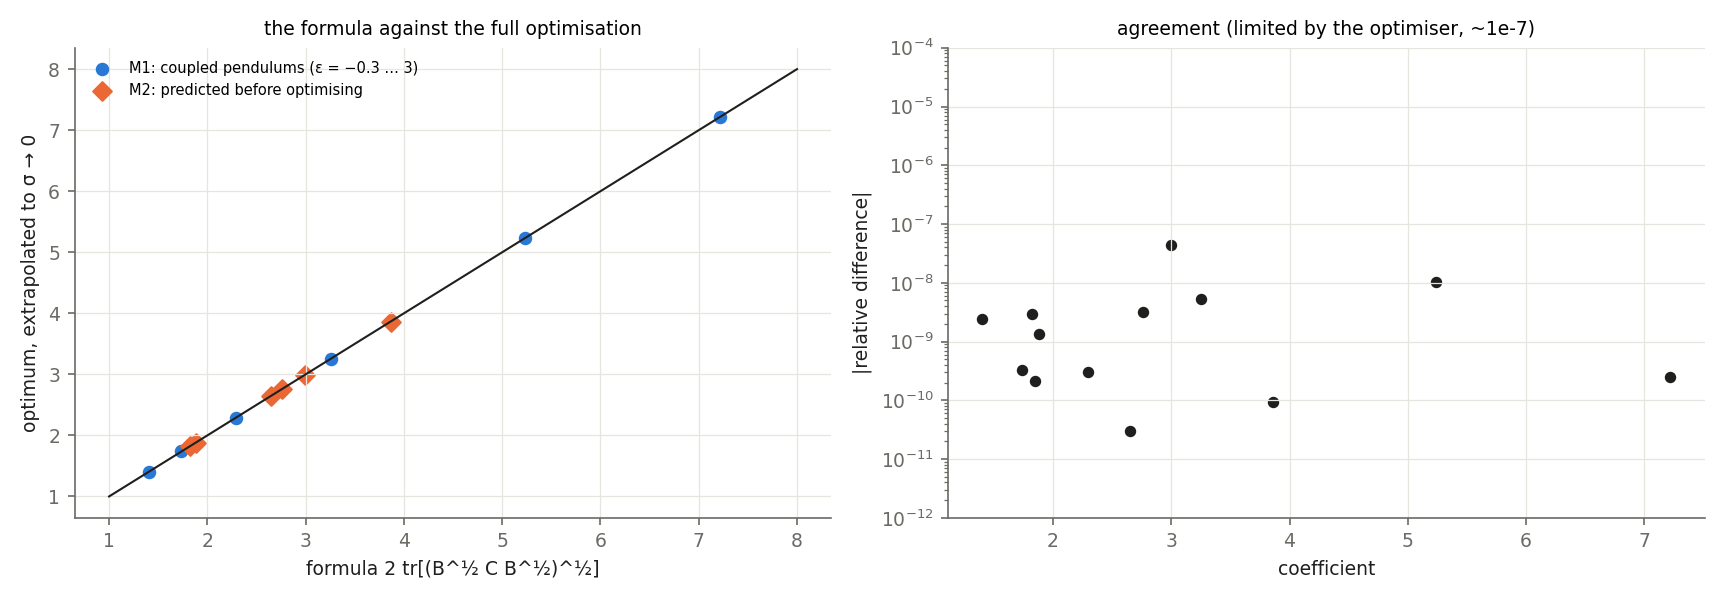
\includegraphics[width=0.95\textwidth]{figures/fig1_formula.png}
\caption{The formula $\Gamma = 2\tr[(B^{1/2}CB^{1/2})^{1/2}]$ against the best Gaussian state found by full optimization, extrapolated to $\sigma \to 0$. Circles: two coupled pendulums, $\varepsilon = -0.3$ to $3$ (Table~\ref{tab:coupled}). Diamonds: systems whose $\Gamma$ was recorded before the optimization (Sec.~\ref{sec:prediction}, Table~\ref{tab:prediction}). Right: relative difference, limited by the precision of the optimizer.}
\label{fig:formula}
\end{figure*}

\emph{The picture.} The observer's eye is a thin needle across the stretching direction of the first pendulum. It must be long in every other direction, but it pays only for the configuration directions on which the maximal strain depends: the contracting partner $w$ of the first pendulum, at the full price $2\kappa$, and the position of the second pendulum, at the price $\kappa$ weighted by the coupling. The second pendulum's momentum is free.

\section{Predictions for other systems}
\label{sec:prediction}

The formula~\eqref{eq:Gamma} was found after the two-pendulum optimum had been seen. To test it as a prediction we computed $\kappa$, $q_0$, $B$ and $\Gamma$ for systems that played no part in its derivation, wrote the predicted values to a file before any optimization of those systems, and recorded the time and a SHA-256 hash of the file (2026-10-13T00:46:28Z; hash beginning \texttt{d84ba44a}). The optimization scripts check the hash before they run. Independently, and without access to that file, the predictions for the chains were computed a second time with a separate implementation; the two agree to seven digits.

The systems are open chains of $n = 3$ and $4$ pendulums,
\begin{equation}
V = -\sum_{i=1}^n \cos q_i - \varepsilon\sum_{i=1}^{n-1}\cos(q_i - q_{i+1}),
\label{eq:chain}
\end{equation}
and two pendulums of different strength with a product coupling,
\begin{equation}
V = -\cos q_1 - 2\cos q_2 - \varepsilon\cos q_1\cos q_2 .
\label{eq:product}
\end{equation}

\begin{table}[t]
\caption{Predictions recorded before optimization. $q_0/\pi$: point of maximal strain; $\Gamma$: predicted coefficient; optimum: best Gaussian state found by full optimization, extrapolated to $\sigma \to 0$ from $\sigma = 10^{-4}, 10^{-5}, 10^{-6}$.}
\label{tab:prediction}
\begin{ruledtabular}
\begin{tabular}{lllll}
system & $q_0/\pi$ & $\kappa$ & $\Gamma$ (predicted) & optimum \\
\hline
chain, $n=3$, $\varepsilon=0.1$ & $(0,1,0)$ & $1.104741$ & $1.8198116$ & $1.8198116$ \\
chain, $n=3$, $\varepsilon=0.3$ & $(0,1,0)$ & $1.337883$ & $2.7601116$ & $2.7601116$ \\
chain, $n=4$, $\varepsilon=0.1$ & $(0,1,0,1)$ & $1.104975$ & $1.8798244$ & $1.8798244$ \\
chain, $n=4$, $\varepsilon=0.3$ & $(0,1,0,1)$ & $1.343139$ & $2.9974827$ & $2.9974828$ \\
product, $\varepsilon=0.3$ & $(0,1)$ & $1.65$ & $2.6516383$ & $2.6516383$ \\
product, $\varepsilon=1$ & $(0,1)$ & $2$ & $3.8637033$ & $3.8637033$ \\
\end{tabular}
\end{ruledtabular}
\end{table}

\begin{observation}[Predictions]
\label{obs:prediction}
All six predictions agree with the optimum to a relative $4\times10^{-8}$ (Table~\ref{tab:prediction}, Fig.~\ref{fig:formula}). The optimization was carried out over all parameters in a frame scaled to the expected widths, from the predicted state and from random perturbations of it; in addition, four random starts per system in the original coordinates were run, and none went below the optimum. In every system the momentum-only directions were free: their width ran to the end of the search range and their share of the Fisher matrix, $\sigma^2 e^{\mathsf T}Fe$, was below $10^{-12}$.
\end{observation}

\emph{How the coefficient grows.} For $\varepsilon = 0.1$, $\Gamma$ is $1.40$, $1.82$ and $1.88$ for $n = 2, 3, 4$. For $n = 3$ the maximal strain sits on the middle pendulum at its top, with both neighbours hanging at the bottom; each neighbour adds roughly $2\sqrt{\kappa B_{kk}}$ for its position, about $0.3$ here. For $n = 4$ the maximum has two pendulums at their tops, and one configuration direction adds only $0.08$: it belongs to a mode that is itself almost as unstable as the top one ($1.0525$ against $\kappa = 1.105$), so spreading along it hardly lowers the maximal strain. The coefficient counts how sensitive the maximal strain is to each configuration direction, not how many directions there are.

\emph{Where the formula does not apply.} For the H\'enon--Heiles potential the eigenvalues of $M$ are $\pm\sqrt{x^2+y^2}$, so the strain grows without bound and has no maximum; the assumption of Sec.~\ref{sec:setting} fails, and we made no prediction. If the phase space is restricted, for instance to an energy shell, the maximum lies on the boundary, where the strain decreases linearly rather than quadratically, and the gap is expected to scale with a different power of $\sigma$; we have not computed it.

\section{Beyond Gaussian states}
\label{sec:mixtures}

For one degree of freedom, Gaussian mixtures beat the best Gaussian state: fans of segments through the point of maximal strain by about $5\%$ of the gap, and irregular bundles of needles found by direct optimization by about $8\%$; the gap stays proportional to $\sigma$~\cite{namba2026gap}. In several degrees of freedom the question is how much of this gain survives.

\emph{States.} We use product states: a mixture of $K$ Gaussians in the plane $(v,w)$ of the most stretching mode, combined with one common Gaussian along the configuration direction $a$ of the other mode, the two coupled by a rotation angle $\theta$, and infinitely broad along the momentum direction $b$. The integral along $a$ is then in closed form, so the critical rate is evaluated on a two-dimensional grid; it agrees with a three-dimensional evaluation to $2\times10^{-6}$, and for a single Gaussian with Eq.~\eqref{eq:gaplaw} to $10^{-6}$. The best Gaussian state belongs to this family. Allowing the shape to leave the family afterwards lowered the gap by a further $0.06\%$ ($\varepsilon = 0.1$) and $0.24\%$ ($\varepsilon = 0.3$) of the Gaussian gap, an order of magnitude less than the gain itself.

\emph{Search.} The single pendulum and the coupled pendulums were searched with the same procedure and effort (random hill climbing followed by L-BFGS), from the best one-degree-of-freedom bundles. For the single pendulum the procedure reaches $0.9188\,\sigma$ at $K = 16$, within $0.3\%$ of the best gap found by long searches.

\begin{table}[t]
\caption{Mixtures against the best Gaussian state, $(\kappa - R)/(\kappa - R^*)$, at $\sigma = 10^{-3}$ with the same search for all three systems. Last two columns: the gain $1 - (\kappa-R)/(\kappa-R^*)$ of the coupled system divided by that of the single pendulum.}
\label{tab:mixtures}
\begin{ruledtabular}
\begin{tabular}{llllll}
$K$ & 1 d.o.f. & $\varepsilon = 0.1$ & $\varepsilon = 0.3$ & gain ratio $0.1$ & gain ratio $0.3$ \\
\hline
2 & 0.9795 & 0.9889 & 0.9925 & 0.54 & 0.37 \\
4 & 0.9529 & 0.9728 & 0.9798 & 0.58 & 0.43 \\
8 & 0.9362 & 0.9655 & 0.9751 & 0.54 & 0.39 \\
16 & 0.9196 & 0.9580 & 0.9694 & 0.52 & 0.38 \\
\end{tabular}
\end{ruledtabular}
\end{table}

\begin{observation}[Mixtures gain less in several degrees of freedom]
\label{obs:mixtures}
In two coupled pendulums the gain of mixtures over the best Gaussian state is about $55\%$ ($\varepsilon = 0.1$) and $40\%$ ($\varepsilon = 0.3$) of the gain in one degree of freedom, at every $K$ from $2$ to $16$ (Table~\ref{tab:mixtures}, Fig.~\ref{fig:mixtures}). Almost all of it, $99\%$ for $\varepsilon = 0.1$ and $90\%$ for $\varepsilon = 0.3$ at $K = 8$, comes from mixing inside the plane $(v,w)$ with the law along $a$ kept as in the best Gaussian state. Mixing in the plane raises the cost along $a$ (by $0.03\%$ and $0.5\%$ of the Gaussian gap at $K = 8$), and the optimal mixture partly compensates by widening the law along $a$ by $4$--$7\%$ and reducing $\theta$.
\end{observation}

If mixtures gained only inside the plane and the other directions merely diluted the gain, the ratio would equal the share $f$ of the plane in $\Gamma$, $0.77$ for $\varepsilon = 0.1$ and $0.71$ for $\varepsilon = 0.3$. The observed ratio is smaller: the gain inside the plane is itself smaller than in one degree of freedom, and the cross term along $a$ costs extra. Empirically the ratio is described by $f^{a}$ with $a \approx 2.6$ (fitted; the individual values lie between $2.1$ and $2.9$). As a test, the ratios for $\varepsilon = 1$ and $\varepsilon = -0.3$ were predicted with this law before they were computed, and the predictions were recorded with time and hash (2026-10-13T09:58:04Z; hash beginning \texttt{96300c58}). The predicted gains were within $6\%$ and $3\%$ of the observed ones; for $\varepsilon = -0.3$ the observed value lies inside the predicted range, for $\varepsilon = 1$ just outside it, with a gain slightly larger than predicted. A model that treated the coupled system as a single pendulum with an effective $\beta$, recorded at the same time, overestimated the gain by a factor $1.4$--$1.9$ and is rejected. The exponent $a$ is not derived.

\begin{figure*}[t]
\centering
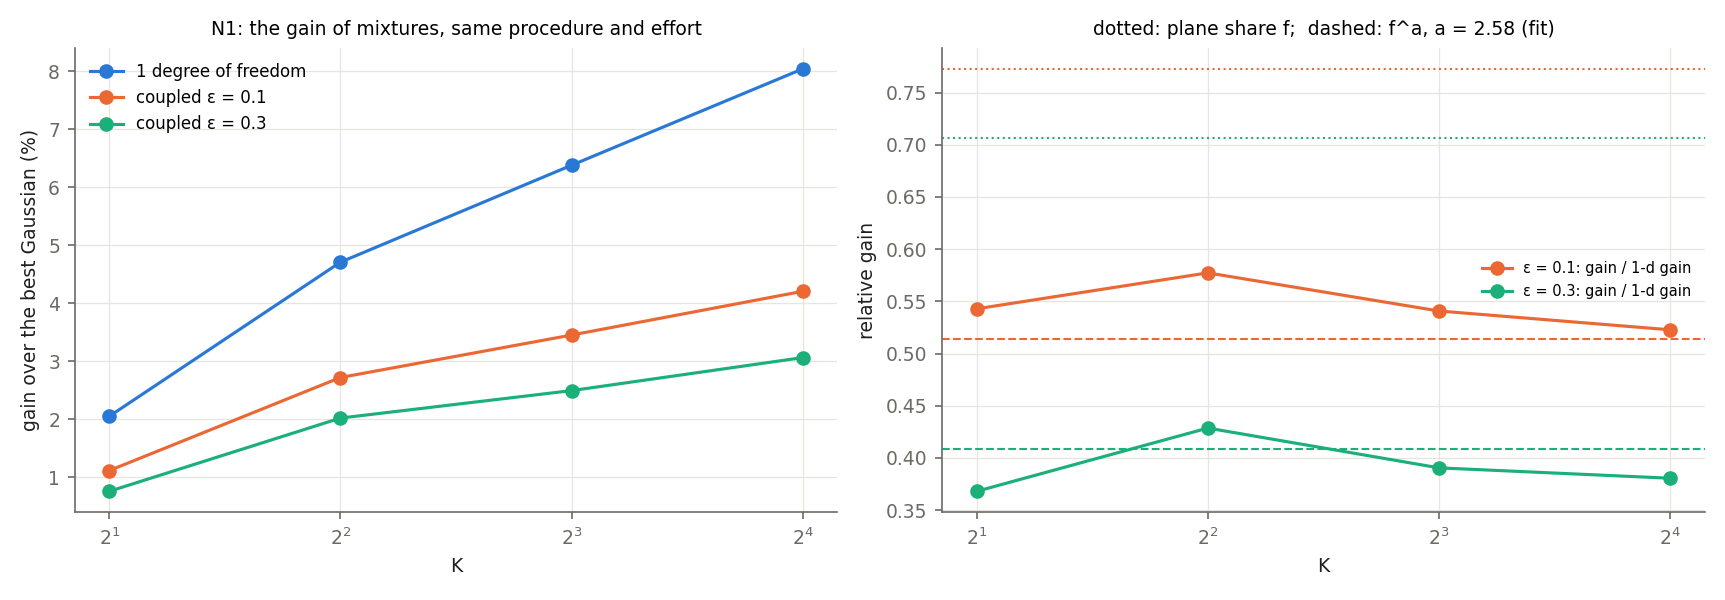
\includegraphics[width=0.95\textwidth]{figures/fig2_mixtures.png}
\caption{Mixtures in one and two degrees of freedom, same search procedure and effort. Left: gain over the best Gaussian state against the number of components $K$. Right: gain of the coupled system divided by that of the single pendulum; dotted lines: share $f$ of the plane $(v,w)$ in $\Gamma$; dashed lines: $f^{a}$ with the fitted $a = 2.58$.}
\label{fig:mixtures}
\end{figure*}

\section{Conclusion}
\label{sec:conclusion}

For mechanical systems with any number of degrees of freedom, the resolution gap of Gaussian states is controlled by a single matrix formula, $\Gamma = 2\tr[(B^{1/2}CB^{1/2})^{1/2}]$. We proved that $\Gamma\sigma$ is an upper bound on the gap of the best Gaussian state, to first order in $\sigma$, and that momentum directions are free. For two coupled pendulums the formula is explicit; in thirteen systems, six of them predicted before they were computed, the best Gaussian state found without any assumed shape matches it in value to a relative $4\times10^{-8}$ and in shape. Mixtures gain less in several degrees of freedom than in one, because their advantage lives in the plane of the most stretching mode and does not extend to the other directions.

The answer to the question of the introduction is that the gap does not grow with the number of degrees of freedom as such. It grows with the number of configuration directions on which the maximal strain depends, each weighted by how strongly it depends on them. An observer focused on one unstable mode can ignore uncoupled modes entirely and all momenta at no cost, and pays for a weakly coupled mode in proportion to the square root of the coupling.

Three questions remain open. The first is Conjecture~\ref{conj:optimal}: a proof that no Gaussian state does better than the family~\eqref{eq:family}. The second is the uniform gap over all states, not only Gaussian ones, which is open already for one degree of freedom~\cite{namba2026gap}. The third concerns flows that are not of the form $|p|^2/2 + V(q)$: there the strain depends on momenta, Proposition~\ref{prop:momentum} fails, and the cost of momentum directions must enter $B$.

The same balance appears in phase-space diffusion models, where a learned score plays the role of the coarse-grained density~\cite{namba2026threshold}. A formula that says which directions of a many-dimensional state are costly and which are free is what such applications need.


\appendix
\section{Proofs}
\label{app:proofs}

\subsection{Lemma~\ref{lem:matrix}}
Put $T = C^{1/2}UC^{1/2}$ and $X = C^{1/2}BC^{1/2} \succeq 0$. Then $\tr(BT) = \tr(XU)$ and $\tr(CT^{-1}) = \tr(U^{-1})$, and
\begin{equation}
\tr(XU) + \tr(U^{-1}) - 2\tr X^{1/2} = \big\|X^{1/2}U^{1/2} - U^{-1/2}\big\|_F^2 \geq 0,
\end{equation}
because the cross term is $\tr(U^{1/2}X^{1/2}U^{-1/2}) = \tr X^{1/2}$. If $X \succ 0$, equality holds for $U = X^{-1/2}$, which gives $T_*$. If $X$ is singular, take $U = (X + \eta I)^{-1/2}$ and let $\eta \to 0$; the left side tends to $2\tr X^{1/2}$. Finally $\tr X^{1/2} = \tr(B^{1/2}CB^{1/2})^{1/2}$, since $C^{1/2}BC^{1/2}$ and $B^{1/2}CB^{1/2}$ have the same nonzero eigenvalues.

\subsection{Theorem~\ref{thm:upper}}
Write $L = (u_1,\dots,u_n)$ and $\Pi = \sum_j b_jb_j^{\mathsf T}$. In the orthonormal frame $(v; u_1,\dots,u_n; b_2,\dots,b_n)$ the covariance~\eqref{eq:family} is block diagonal, with blocks $0$, $\sigma T$ and $I_{n-1}$, so
\begin{equation}
F = \sigma^{-2}vv^{\mathsf T} + \sigma^{-1}L(T + \sigma I)^{-1}L^{\mathsf T} + (1+\sigma^2)^{-1}\Pi,
\end{equation}
and $\tr\big(F(\kappa I - K)\big)$ is the sum of the three block traces.

\emph{The $v$ block.} $v^{\mathsf T}Kv = e_+^{\mathsf T}\bar Me_+ = \E[g(q)]$ with $q \sim \mathcal N(q_0, S_{qq})$ and $S_{qq} = \sigma PTP^{\mathsf T}$. Since $g$ is built from $V''$, its $k$-th derivative involves $V^{(k+2)}$, so under the assumption of Sec.~\ref{sec:setting} $g$ has four continuous bounded derivatives. Taylor's theorem to fourth order, with $\nabla g(q_0) = 0$ and vanishing odd moments, gives $\E[g(q)] = \kappa - \tr(B_qS_{qq}) + r$ with $|r| \leq \tfrac1{24}\sup\|\nabla^4 g\|\,\E|q-q_0|^4 \leq \tfrac18\sup\|\nabla^4 g\|\,(\tr S_{qq})^2$, using $\E|x|^4 = (\tr S)^2 + 2\tr S^2 \leq 3(\tr S)^2$ for $x \sim \mathcal N(0,S)$. Hence $\kappa - v^{\mathsf T}Kv = \sigma\tr(BT) + O(\sigma^2)$. If $V$ has only four continuous bounded derivatives, $g$ has two, and Taylor's theorem to second order with dominated convergence gives $r = o(\tr S_{qq})$ instead; the rest of the proof uses only $V^{(4)}$, so Eq.~\eqref{eq:upper} still holds, with $o(\sigma)$ in place of $O(\sigma^2)$.

\emph{The $u$ block.} $w^{\mathsf T}Kw = -e_+^{\mathsf T}\bar Me_+ = -\kappa + O(\sigma)$; $w^{\mathsf T}Ka_j = -e_+^{\mathsf T}\bar Me_j/\sqrt2 = O(\sigma)$, because $e_+^{\mathsf T}M(q_0)e_j = 0$ and $\bar M - M(q_0) = O(\|S_{qq}\|)$; $a_i^{\mathsf T}Ka_j = 0$. So $\kappa I - L^{\mathsf T}KL = C + O(\sigma)$, and the block contributes $\sigma^{-1}\tr(T^{-1}C) + O(1)$.

\emph{The $b$ block.} $b_i^{\mathsf T}Kb_j = 0$, so it contributes $(n-1)\kappa/(1+\sigma^2) = O(1)$.

Together, $\tr(F(\kappa I - K)) = \sigma^{-1}[\tr(BT) + \tr(CT^{-1})] + O(1)$ and $\tr F = \sigma^{-2}(1 + O(\sigma))$, which is Eq.~\eqref{eq:familygap}. Here $T$ is fixed as $\sigma \to 0$, and the constants in the $O(\cdot)$ terms depend on $T$ through $\|T\|$ and $\|T^{-1}\|$ (for instance $(T + \sigma I)^{-1} = T^{-1} + O(\sigma\|T^{-1}\|^2)$), but not on $\sigma$.

To conclude, note that the state~\eqref{eq:family} is singular, with zero width along $v$; by Sec.~\ref{sec:setting} it is admissible, and at each fixed $\sigma$ it is the limit of non-degenerate states with the same limit of $R$, so $R^* \geq R$ for it. If $B \succ 0$, take $T = T_*$: then $\kappa - R^* \leq \sigma\,\Gamma + O(\sigma^2)$ with a constant depending only on $T_*$. If $B$ is singular, for every $\delta > 0$ choose a fixed $T_\delta \succ 0$ with $\tr(BT_\delta) + \tr(CT_\delta^{-1}) \leq \Gamma + \delta$, which exists by Lemma~\ref{lem:matrix}. Then $\limsup_{\sigma\to0}(\kappa - R^*)/\sigma \leq \Gamma + \delta$, and letting $\delta \to 0$ after $\sigma \to 0$ gives Eq.~\eqref{eq:upper}. The two limits are taken in this order, so the $T$-dependence of the constants is harmless.

Two remarks. The width of the state along the $b_j$ can be any fixed number; its contribution is $O(\sigma^2)$ to the gap. The tilt of the optimal segment towards $-v$ found in one degree of freedom~\cite{namba2026gap} is a correction of order $\sigma^2$ and does not enter at this order.

\subsection{Weak-coupling series}
\label{app:series}
For the potential~\eqref{eq:coupledV}, $\kappa = 1 + \varepsilon/2 + \varepsilon^2/4 + O(\varepsilon^4)$ and $e_+ = (1 - \varepsilon^2/8, -\varepsilon/2) + O(\varepsilon^3)$, so $d = 1 + \varepsilon + O(\varepsilon^3)$ and
\begin{equation}
4B_q = \begin{pmatrix} 1 + \varepsilon + \tfrac34\varepsilon^2 & -\varepsilon - \varepsilon^2 \\ -\varepsilon - \varepsilon^2 & \varepsilon + \tfrac34\varepsilon^2\end{pmatrix} + O(\varepsilon^3).
\end{equation}
Projecting on $P$ gives the entries of $B$ in Eq.~\eqref{eq:coupledseries}. With $X = C^{1/2}BC^{1/2}$, $\tr X = \tfrac14 + \tfrac58\varepsilon + O(\varepsilon^2)$ and $\det X = \tfrac{\varepsilon}{16}(1 + \tfrac74\varepsilon) + O(\varepsilon^3)$. For a $2\times2$ matrix $\tr X^{1/2} = (\tr X + 2\sqrt{\det X})^{1/2}$, so
\begin{equation}
\Gamma = \big(1 + 2\sqrt\varepsilon + \tfrac52\varepsilon + \tfrac74\varepsilon^{3/2} + O(\varepsilon^2)\big)^{1/2},
\end{equation}
which expands to Eq.~\eqref{eq:coupledseries}. Against the exact $\Gamma$, the truncation error is $9.4\times10^{-7}$ at $\varepsilon = 10^{-3}$, $9.6\times10^{-9}$ at $10^{-4}$ and $9.7\times10^{-11}$ at $10^{-5}$; divided by $\varepsilon^2$ it tends to $0.97$, as it must for an $O(\varepsilon^2)$ remainder.

\section{Numerical methods and verification}
\label{app:methods}

\emph{Gaussian states.} By Eq.~\eqref{eq:gaplaw}, the critical rate of a Gaussian state needs only $\bar M$, which for trigonometric potentials is a closed form: $\E\cos q_i = \cos m_i\,e^{-S_{ii}/2}$ and $\E\cos(q_1-q_2) = \cos(m_1-m_2)\,e^{-(S_{11}+S_{22}-2S_{12})/2}$. Eq.~\eqref{eq:gaplaw} was checked against two evaluations that do not use it: a four-dimensional Gauss--Hermite grid ($18^4$ points) for the posterior-mean form of $R$, and Monte Carlo with $4\times10^6$ samples. On nine random states ($\varepsilon = 0, 0.1, 0.3$) the grid agrees to $10^{-10}$ and Monte Carlo within $2.4$ standard errors.

\emph{Small $\sigma$.} For states that are very long along $b$ and thin along $v$, $(S + \sigma^2 I)^{-1}$ is evaluated in a frame scaled by $(\sigma, \sqrt\sigma, \sqrt\sigma, 1)$ along $(v, w, a, b)$, which keeps full precision down to $\sigma = 10^{-7}$.

\emph{The matrix $B$.} The closed form~\eqref{eq:coupledBq} agrees with a finite-difference evaluation of $\lambda_{\max}(\bar M)$ in $S_{qq}$ to seven digits for $10^{-4} \leq \varepsilon \leq 1$, and an independent implementation of the family~\eqref{eq:family} reproduces $\Gamma$ to $10^{-4}$ at $\sigma = 10^{-6}$.

\emph{Optimization.} The law~\eqref{eq:gaplaw} is evaluated without forming $S + \sigma^2 I$: $\tr F$ and $\tr(FK)$ are obtained from a QR decomposition of $[L^{\mathsf T}; \sigma I]$ with $S = LL^{\mathsf T}$, which keeps full precision for eigenvalues of $S$ between $0$ and $10^8$ and $\sigma$ down to $10^{-7}$. Searches without an assumed shape use the full $n\times n$ factor $L$ in the original coordinates and follow the optimum down in $\sigma$ from $10^{-1}$; a first version with a lower-triangular factor and logarithmic diagonal stalled on flat regions and was replaced. Optima in a frame scaled to the expected widths, from several starts, give the extrapolations to $\sigma\to0$ (quadratic in $\sigma$ through $10^{-4}, 10^{-5}, 10^{-6}$).

\emph{Prediction protocol.} The predictions of Table~\ref{tab:prediction} were written by a script that computes $\kappa$, $q_0$ (from 400 starts and a $1441^2$ grid where applicable) and $B$, before any optimization of those systems; the file was made read-only and its SHA-256 hash and time logged, and the optimization scripts verify the hash. The verification suite checks the hash and recomputes the predictions from their definitions.

\emph{Independent checks.} The following were recomputed with code written separately: $\Gamma$ for all thirteen systems from a numerical Hessian of $e_+^{\mathsf T}V''e_+$ (agreement $2\times10^{-7}$); the predictions for the chains (seven digits); a shape-free search for $\varepsilon = 0.1, 0.3$ with a different parametrization; Lemma~\ref{lem:matrix} on random matrices; Theorem~\ref{thm:upper} with the exact block form of $F$; Proposition~\ref{prop:momentum}; and the series~\eqref{eq:coupledseries}.

\emph{Verification.} Every number of this article is checked by scripts in the repository given below. The verification suite of the numerical study has $479$ checks (stages A--N, of which $198$ belong to stages L--N, the work for this article), and the independent checks of the analytical statements add $64$. All pass. Each check of the study states its tolerance and reports the fraction of it that is used; none uses more than $20\%$.


\section*{Acknowledgments}
The author used AI assistants in this work: Google Gemini (\mbox{Gemini 3.8 Flash}) and OpenAI ChatGPT (\mbox{GPT-5.6 Luna}), for independent cross-checking and critical reading of the draft, and Anthropic Claude (\mbox{claude-opus-5-5}), in two separate sessions. In the first session it took part in theoretical discussion, derived the closed form~\eqref{eq:Bq} of the strain-decay matrix, Proposition~\ref{prop:momentum}, Theorem~\ref{thm:upper} and the series~\eqref{eq:coupledseries}, wrote independent numerical checks, and drafted the text. In the second session it designed and ran the numerical study, wrote the evaluation and verification code, and found the matrix formula~\eqref{eq:Gamma} from the numerical optimum. Results were passed between the sessions as written summaries and checked in the first session by re-running the verification suite and by independent methods. The author directed the research, made all decisions on its content, and takes full responsibility for this article.

\section*{Data and Code Availability}
Scripts that reproduce every analytical statement, number and figure of this article, together with the verification suite, are openly available at \url{https://github.com/neginyan/resolution-gap-many-dof}. \pending{Zenodo DOI of the code version used for this article.}


\begin{thebibliography}{99}

\bibitem{namba2026arrow}
T.~Namba, \textit{Sharp criterion for the coarse-grained arrow of time in Hamiltonian dynamics}, preprint, version v1.2, Zenodo (2026), \href{https://doi.org/10.5281/zenodo.23258135}{doi:10.5281/zenodo.23258135}.

\bibitem{namba2026gap}
T.~Namba, \textit{A resolution gap for the coarse-grained arrow of time in nonlinear Hamiltonian flows}, preprint, version v1.1, Zenodo (2026), \href{https://doi.org/10.5281/zenodo.23320603}{doi:10.5281/zenodo.23320603}.

\bibitem{namba2026threshold}
T.~Namba, \textit{A stretching-rate threshold for phase-space diffusion models with isotropic marginal noise schedules}, preprint, Zenodo (2026), \href{https://doi.org/10.5281/zenodo.23181225}{doi:10.5281/zenodo.23181225}.

\end{thebibliography}


\end{document}
